\documentclass[output=paper,modfonts,nonflat]{langsci/langscibook} 
\author{Ana Regina Calindro\affiliation{}}
\title{Ditransitive constructions: what sets Brazilian Portuguese apart from other Romance languages?}

\abstract{}
\IfFileExists{../localcommands.tex}{
  % add all extra packages you need to load to this file  
\usepackage{tabularx} 
\usepackage{url} 
\urlstyle{same}

\usepackage{listings}
\lstset{basicstyle=\ttfamily,tabsize=2,breaklines=true}


%%%%%%%%%%%%%%%%%%%%%%%%%%%%%%%%%%%%%%%%%%%%%%%%%%%%
%%%                                              %%%
%%%           Examples                           %%%
%%%                                              %%%
%%%%%%%%%%%%%%%%%%%%%%%%%%%%%%%%%%%%%%%%%%%%%%%%%%%% 
%% to add additional information to the right of examples, uncomment the following line
% \usepackage{jambox}
%% if you want the source line of examples to be in italics, uncomment the following line
% \renewcommand{\exfont}{\itshape}
\usepackage{langsci-optional}
\usepackage{./langsci/styles/langsci-gb4e}
\usepackage{./langsci/styles/langsci-lgr}
\usepackage{pgfplots,pgfplotstable}

\definecolor{lsDOIGray}{cmyk}{0,0,0,0.45}

\usepackage{xassoccnt}
\newcounter{realpage}
\DeclareAssociatedCounters{page}{realpage}
\AtBeginDocument{%
  \stepcounter{realpage}
}


 



 

  \newcommand{\appref}[1]{Appendix \ref{#1}}
\newcommand{\fnref}[1]{Footnote \ref{#1}} 

\newenvironment{langscibars}{\begin{axis}[ybar,xtick=data, xticklabels from table={\mydata}{pos}, 
        width  = \textwidth,
	height = .3\textheight,
    	nodes near coords, 
	xtick=data,
	x tick label style={},  
	ymin=0,
	cycle list name=langscicolors
        ]}{\end{axis}}
        
\newcommand{\langscibar}[1]{\addplot+ table [x=i, y=#1] {\mydata};\addlegendentry{#1};}

\newcommand{\langscidata}[1]{\pgfplotstableread{#1}\mydata;}

\makeatletter
\let\thetitle\@title
\let\theauthor\@author 
\makeatother

\newcommand{\togglepaper}[1][0]{ 
%   \bibliography{../localbibliography}
  \papernote{\scriptsize\normalfont
    \theauthor.
    \thetitle. 
    To appear in: 
    Change Volume Editor \& in localcommands.tex 
    Change volume title in localcommands.tex
    Berlin: Language Science Press. [preliminary page numbering]
  }
  \pagenumbering{roman}
  \setcounter{chapter}{#1}
  \addtocounter{chapter}{-1}
}
\newcommand{\orcid}[1]{}
 
  %% hyphenation points for line breaks
%% Normally, automatic hyphenation in LaTeX is very good
%% If a word is mis-hyphenated, add it to this file
%%
%% add information to TeX file before \begin{document} with:
%% %% hyphenation points for line breaks
%% Normally, automatic hyphenation in LaTeX is very good
%% If a word is mis-hyphenated, add it to this file
%%
%% add information to TeX file before \begin{document} with:
%% %% hyphenation points for line breaks
%% Normally, automatic hyphenation in LaTeX is very good
%% If a word is mis-hyphenated, add it to this file
%%
%% add information to TeX file before \begin{document} with:
%% \include{localhyphenation}
\hyphenation{
affri-ca-te
affri-ca-tes
Tarra-go-na
Vio-le-ta
Jacken-doff
clit-ics
Giar-di-ni
Mor-fo-sin-tas-si
mi-ni-mis-ta
nor-ma-li-tza-ció
Caus-ees
an-a-phor-ic
caus-a-tive
caus-a-tives
Mar-antz
ac-cu-sa-tive
Ma-no-les-sou
phe-nom-e-non
Holm-berg
}

\hyphenation{
affri-ca-te
affri-ca-tes
Tarra-go-na
Vio-le-ta
Jacken-doff
clit-ics
Giar-di-ni
Mor-fo-sin-tas-si
mi-ni-mis-ta
nor-ma-li-tza-ció
Caus-ees
an-a-phor-ic
caus-a-tive
caus-a-tives
Mar-antz
ac-cu-sa-tive
Ma-no-les-sou
phe-nom-e-non
Holm-berg
}

\hyphenation{
affri-ca-te
affri-ca-tes
Tarra-go-na
Vio-le-ta
Jacken-doff
clit-ics
Giar-di-ni
Mor-fo-sin-tas-si
mi-ni-mis-ta
nor-ma-li-tza-ció
Caus-ees
an-a-phor-ic
caus-a-tive
caus-a-tives
Mar-antz
ac-cu-sa-tive
Ma-no-les-sou
phe-nom-e-non
Holm-berg
}

  \bibliography{../localbibliography}
  \togglepaper[1]%%chapternumber
}{}

\begin{document}
\maketitle 


\textbf{Ditransitive} \textbf{constructions:} \textbf{what} \textbf{sets} \textbf{Brazilian} \textbf{Portuguese} \textbf{apart} \textbf{from} \textbf{other} \textbf{Romance} \textbf{languages?}

\textbf{Ana} \textbf{Calindro}

\textbf{Federal} \textbf{University} \textbf{of} \textbf{Rio} \textbf{de} \textbf{Janeiro} \textbf{(UFRJ)}

\textbf{\textit{Abstract}}. \textit{The} \textit{aim} \textit{of} \textit{this} \textit{paper} \textit{is} \textit{to} \textit{discuss} \textit{whether} \textit{a} \textit{particular} \textit{diachronic} \textit{change} \textit{in} \textit{the} \textit{expression} \textit{of} \textit{indirect} \textit{objects} \textit{(IOs)} \textit{in} \textit{Brazilian} \textit{Portuguese} \textit{(BP)} \textit{has} \textit{set} \textit{this} \textit{language} \textit{apart} \textit{from} \textit{other} \textit{Romance} \textit{languages.} \textit{Since} \textit{the} \textit{19\textsuperscript{th}} \textit{century,} \textit{BP} \textit{has} \textit{been} \textit{generalizing} \textit{the} \textit{use} \textit{of} \textit{the} \textit{preposition} para \textit{‘to’} \textit{in} \textit{ditransitive} \textit{sentences} \textit{with} \textit{verbs} \textit{of} \textit{movement,} \textit{transfer} \textit{and} \textit{creation.} \textit{Moreover,} \textit{the} \textit{morphological} \textit{counterpart} \textit{of} \textit{the} \textit{dative} \textit{argument} \textit{in} \textit{the} \textit{third} \textit{person} \textit{(the} \textit{clitic} lhe(s)) \textit{has} \textit{been} \textit{replaced} \textit{by} \textit{other} \textit{strategies,} \textit{while} \textit{in} \textit{European} \textit{Portuguese} \textit{(EP),} \textit{IOs} \textit{in} \textit{the} \textit{same} \textit{contexts} \textit{are} \textit{introduced} \textit{by} \textit{the} \textit{dummy} \textit{preposition} \textit{a} \textit{and} \textit{can} \textit{always} \textit{alternate} \textit{with} lhe(s). \textit{According} \textit{to} \textit{Torres} \textit{\citet{Morais2007}, these IOs in EP are dative arguments introduced by an applicative head, as also argued by \citet{Cuervo2003} for Spanish, and \citet{DiaconescuRivero2007} for Romanian.}\textbf{ }\textit{In} \textit{this} \textit{paper,} \textit{I} \textit{will} \textit{propose} \textit{that} \textit{the} \textit{ditransitive} \textit{sentences} \textit{in} \textit{BP} \textit{have} \textit{a} \textit{different} \textit{structural} \textit{representation} \textit{from} \textit{other} \textit{Romance} \textit{languages,} \textit{given} \textit{that} \textit{it} \textit{cannot} \textit{express} \textit{dative} \textit{case} \textit{in} \textit{the} \textit{third} \textit{person} \textit{anymore,} \textit{nor} \textit{via} \textit{functional} \textit{prepositions,} \textit{nor} \textit{by} \textit{the} \textit{clitic} lhe(s). \textit{Consequently,} \textit{I} \textit{propose} \textit{that} \textit{the} \textit{IOs} \textit{in} \textit{BP} \textit{should} \textit{be} \textit{introduced} \textit{via} \textit{a} \textit{p} \textit{head,} \textit{based} \textit{on} \textit{the} \textit{proposals} \textit{of} \textit{Svenonius} \textit{(2003,} \textit{2004),} \textit{\citet{Wood2012} and the i* single argument introducer proposal by \citet{WoodMarantz2017}.}

\textbf{Keywords:} \textit{ditransitive} \textit{sentences,} \textit{Case} \textit{assignment,} \textit{prepositional} \textit{heads,} \textit{Brazilian} \textit{Portuguese.}

\textbf{1.} \textbf{Introduction} 

The aim of this paper is to discuss whether a diachronic change in the expression of indirect objects (IOs) in Brazilian Portuguese (BP) has set this language apart from other Romance languages, in terms of how IOs are structured.

Since the 19\textsuperscript{th} century, BP has been generalizing the use of full prepositions as \textit{para} ‘to’ in ditransitive sentences with verbs of transfer and movement (cf. 1) and creation (cf. 2) (cf. \citealt{Freire2005}; Torres \citealt{MoraisBerlinck2006}; Torres \citealt{MoraisSalles2010}).

\begin{styleBodyTextii}
\ea%1
    \label{ex:key:1}
    \gll\\
        \\
    \glt
    \z

         Maria enviou  uma carta  \textit{para/} \textit{a}           \textit{o} \textit{João}               / \textit{para} \textit{ele.}    
\end{styleBodyTextii}

\begin{styleBodyTextii}
     Maria sent       a letter      P \textit{\textsubscript{para} \textit{(to)}}/ \textit{\textsubscript{a} \textit{(to)}}   the João. OBL  / to him.3SG  
\end{styleBodyTextii}

\ea%2
    \label{ex:key:2}
    \gll\\
        \\
    \glt
    \z

         Maria     preparou  o jantar        \textit{para}    \textit{o} \textit{João}  / \textit{para} \textit{ele.}        

      Maria     prepared  the dinner    P\textsubscript{para(to)} the João.OBL / for him. 3SG 

In addition, the third person dative argument counterpart (clitic \textit{lhe(s)}) has been replaced in BP by other strategies, such as 3\textsuperscript{rd} person pronouns preceded by \textit{para}:  \textit{para} \textit{ele(s)/} \textit{ela(s)} ‘to him/ her/ them’, as we can see in the examples above.

\begin{styleBodyTextii}
Conversely, in the relevant context, IOs in European Portuguese (EP) are introduced by the preposition \textit{a} and can always alternate with \textit{lhe(s)}.
\end{styleBodyTextii}

\begin{styleBodyTextii}
\ea%3
    \label{ex:key:3}
    \gll\\
        \\
    \glt
    \z

         A    Maria enviou uma carta \textit{ao} \textit{João}            /enviou-\textit{lhe}          uma carta. 
\end{styleBodyTextii}

\begin{styleBodyTextii}
       The Maria sent     a letter      P\textsubscript{} \textit{\textsubscript{a} \textit{(to)}} the João. DAT  / sent -3SG.DAT  a letter.  
\end{styleBodyTextii}

Regarding argument structure representation, ditransitive constructions have always been a challenge for Chomsky’s (1981, 1986) binary-branching model. The two first attempts to deal with the issue were \citegen{Baker1988} incorporation hypothesis and \citegen{Larson1988} VP shells proposal for the Prepositional Dative Construction (PDC) ‘Mary gave a book to John’ and the Double Object Construction (DOC) ‘Mary gave John a book’ in English. This phenomenon is known as the \textit{dative} \textit{alternation.} 

Conversely, \citet{Marantz1993} proposes an applicative head to introduce IOs in DOCs, building on the analysis of Bantu languages, which accounted for the absence of prepositions in DOCs (cf. \citealt{AlsinaMchombo1993}). Following this work, \citet{Pylkkännen2002} established there are two types of applicative constructions (low and high applicatives), which are able to explain different semantics conveyed by IOs in certain ditransitive sentences. 

Based on these proposals, \citet{Cuervo2003} and \citet{DiaconescuRivero2007} show Spanish and Romanian also have the \textit{dative} \textit{alternation}. These analyses, however, differ from the ones for English ditransitives – which are based on the presence or absence of a preposition. According to the aforementioned authors, the \textit{dative} \textit{alternation} in Romance languages depends on the presence or absence of the clitic in the structure\footnote{\textrm{For an alternative perspective, cf. Cépeda \& Cyrino (this volume), who assume structures with} \textrm{\textit{give}}\textrm{{}-type verbs in Spanish, EP and BP are not DOCs. The authors claim dative clitics do not play any role in determining the structural position of DO and IO in these constructions.}}. Hence, in Spanish and Romanian, the DOC is characterized by the IO being doubled by a dative clitic, which is the head of ApplP (cf. 4 and 5):

\ea%4
    \label{ex:key:4}
    \gll\\
        \\
    \glt
    \z

         a. Pablo \textit{le}               mandó un diccionario  \textit{a} \textit{Gabi.} 

           Pablo 3SG.DAT  sent      a dictionary     to Gabi.DAT 

       a’. [\textsubscript{VoiceP} Pablo [\textit{\textsubscript{v’}} voice [\textsubscript{VP} mandó [\textsubscript{ApplP} a Gabi [\textsubscript{APPL’} \textit{le} [\textsubscript{DP} un diccionario]]]]]]                        \citep[35]{Cuervo2003} 

\ea%5
    \label{ex:key:5}
    \gll\\
        \\
    \glt
    \z

         a. Mihaela  \textit{îi}             trimite   \textit{Mari}\textbf{\textit{ei}        }o scrisoare. 

           Mihaela  DAT.CL  sends   Mary.DAT  a letter 

        a'. [\textsubscript{VoiceP} Mihaela [\textit{\textsubscript{v’}} voice [\textsubscript{VP} trimite [\textsubscript{ApplP} Mariei [\textsubscript{APPL’} îi [\textsubscript{DP} o scrisoare]]]]]]                       (\citealt{DiaconescuRivero2007}: 2) 

Configurations (5a’) and (6a’) show the dative argument in SpecApplP. The DO is licensed as its complement and ApplP is the complement of the verb. Therefore, following \citet{Pylkkänen2002}, the applicative head below the verbal root accounts for the \textit{low} \textit{applicative} – which is responsible for relating two DPs that establish a relation of direct transfer of possession. As we can see in (5a’) and (6a’), the clitic is the Spell-out of ApplP, as it is responsible for lexicalizing the DP person and number features in SpecApplP. 

Additionally, the DOC in Spanish is characterized in terms of the IO being accompanied by a preposition (\textit{a} \textit{Gabi/} \textit{a-DP}), which is a dummy element responsible for assigning dative Case to its argument. This IO is necessarily doubled by a dative clitic. 

For Romanian, \citet{DiaconescuRivero2007} present two DOC examples \REF{ex:key:5} and \REF{ex:key:6}, the latter is similar to \REF{ex:key:4} in Spanish, as the dative IO (\textit{la} \textit{Maria}) is doubled by the dative clitic (\textit{îi}).

\ea%6
    \label{ex:key:6}
    \gll\\
        \\
    \glt
    \z

         Mihaela \textit{îi}               trimite   \textit{la} \textit{Maria}          o scrisoare.

     Mihaela DAT. CL  sends     to Maria.DAT  a letter.

      (\citealt{DiaconescuRivero2007}: 14)

According to the authors, sentence \REF{ex:key:6} is not part of the grammar of all speakers of Romanian. However, this example added to the assumption that when IOs are doubled by clitics in Romance languages, they are actually a-DP, not PP. 

Pursuing the idea that clitics paired with IOs, which are actually a-DPs, is the key to understanding the \textit{dative} \textit{alternation} in Romance, Torres \citet{Morais2007} assumes EP also presents this phenomenon. In sentences like \REF{ex:key:3}, the preposition \textit{a} in EP would also be a functional element responsible for assigning dative Case to DPs, as \citet{Cuervo2003} proposes for Spanish (cf.4). Consequently, the possibility of replacing the IO by a dative clitic suggests this element is the morphological expression of the dative case introduced in SpecApplP as a proper argument (cf. 7). 

\begin{styleBodyTextii}
\ea%7
    \label{ex:key:7}
    \gll\\
        \\
    \glt
    \z

         [\textit{\textsubscript{v}}\textsubscript{P} O João [\textit{\textsubscript{v}}\textsubscript{’}\textit{v} [\textsubscript{VP} enviou [\textsubscript{ApplP} à Maria/lhe [\textsubscript{APPL’} Ø [\textsubscript{DP} uma carta]]]]]]]  
\end{styleBodyTextii}

\begin{styleBodyTextii}
                                                                                                (Torres \citealt{Morais2007}: 175)
\end{styleBodyTextii}

Another important fact for the dative alternation in EP is when the IO is introduced by \textit{para}, with pure locatives for instance, it cannot alternate with the dative clitic \textit{lhe(s):}

\ea%8
    \label{ex:key:8}
    \gll\\
        \\
    \glt
    \z

          A Maria     enviou (*lhe)      uma carta  \textit{para} \textit{Lisboa}.

       The Maria sent (3SG.DAT)  a letter      P\textit{\textsubscript{para(to)}} Lisbon.OBL

 (Torres \citealt{Morais2007}:96)

Therefore, sentence \REF{ex:key:8} is considered a Prepositional Dative Construction (PDC) by Torres \citet{Morais2007}. Additionally, in Spanish, \citet{Cuervo2003} considers \REF{ex:key:9} a PDC, because preposition \textit{a} is not doubled by the dative clitic. Hence, the IO is introduced by a proper preposition that assigns oblique Case to its complement

\ea%9
    \label{ex:key:9}
    \gll\\
        \\
    \glt
    \z

         Pablo mandó un diccionario  \textit{a} \textit{Barcelona}.

       Pablo  sent      a dictionary     P \textit{a(to)} Barcelona.OBL

           \citep[36]{Cuervo2003}

If the presence of dative clitics is the main argument to support the idea that Romance languages have the \textit{dative} \textit{alternation}, it is worth noting that BP has been undergoing a diachronic change regarding its pronominal system since the 18\textsuperscript{th} century. This is associated with the loss of third person clitics (cf. \citealt{CarvalhoCalindro2018}), as well as several changes in the prepositions used to introduce IOs, as we will discuss further in this paper. These two facts combined are the central idea for assuming BP seems to be setting different parameters from other Romance languages concerning Case assignment.

On this basis, given this pronominal system reconfiguration in BP, I assume this language is undergoing a change related to Case assignment, because dative case cannot be assigned via a functional preposition any longer (preposition \textit{a}), nor by its 3\textsuperscript{rd} person morphological counterpart (\textit{lhe(s)).} Consequently, BP seems to be shifting from a type of language, which had morphological case for all persons in the accusative and the dative, as EP still does, to one where Case has to be assigned via lexical prepositions.

In order to answer my main research question focusing on the differences between BP and the other Romance languages exemplified, I will analyze how BP expresses IOs both in the pronominal and prepositional phrase forms using data from previous works. First, through the analysis of the Brazilian pronominal system, which has been undergoing several changes since the 18\textsuperscript{th} century \citep{KatoEtAl2009}. Next, based on Calindro (2015, 2016), I will show the prepositions that introduce IOs with transfer/movement and creation verbs in BP have a different status from the ones in Spanish, Romanian and EP. Hence, the structural representation of IOs in BP should be different from the other Romance languages analyzed, once the items involved in these structures have different status.

Bearing these facts in mind, this paper is structured as follows: \sectref{sec:key:2} analyses in more details the variation and change that BP has undergone, in \sectref{sec:key:2.1} regarding the pronominal system and in \sectref{sec:key:2.2} regarding the prepositions that introduce IOs in BP; in \sectref{sec:key:3}, I propose a theoretical account of the sentences with verbs of transfer and movement in BP with a pP head and the universal i* introducer (cf. \citealt{Wood2012}; \citealt{WoodMarantz2017}); in \sectref{sec:key:3.2}, I present a similar proposal for sentences with creation verbs; and finally, in \sectref{sec:key:4}, conclusions are presented.

\textbf{2.} \textbf{Diachronic} \textbf{change} \textbf{in} \textbf{ditransitive} \textbf{sentences} \textbf{in} \textbf{BP}

The pronominal system in BP has undergone modifications since the 18\textsuperscript{th} century (cf. \citealt{KatoEtAl2009}). The table below shows the change for accusative and dative paradigms. The accusative data was adapted from \citet[246]{KatoEtAl2009}, the dative paradigm was added based on \citet{Calindro2015} and Torres \citet{MoraisBerlinck2006} who have observed the loss of the clitic \textit{lhe} in Portuguese from São Paulo state, as well as the work of \citet{Berlinck1997} for Curitiba, \citet{Silveira1999} for \citet{FlorianopolisFreire2005} for Rio de Janeiro.\footnote{\textrm{The dative clitic} \textrm{\textit{lhe}} \textrm{is still active in some areas of Brazil, but it was re-categorized as second person (cf. Figueiredo \citealt{Silva2007}).}}

\tablefirsthead{}

\tabletail{}
\tablelasttail{}
\begin{tabularx}{\textwidth}{XXXXXX} &  & \multicolumn{2}{X}{{\bfseries 19\textsuperscript{th} Century}} & \multicolumn{2}{X}{{\bfseries 20\textsuperscript{th} Century}}\\
\lsptoprule
& \textbf{\textit{Nominative}} & \textbf{\textit{Accusative}} & \textbf{\textit{Dative}} & \textbf{\textit{Accusative}} & \textbf{\textit{Dative}}\\
{\bfseries 1\textsuperscript{st} } & eu & me & me & me & me\\
{\bfseries 2\textsuperscript{nd}}  & (tu) & te & te & te & te\\
{\bfseries 3\textsuperscript{rd}}  & ele (a) & o/a & lhe & \_\_\_ & \_\_\_\\
{\bfseries 1\textsuperscript{st}}  & nós & nos & nos & nos & nos\\
{\bfseries 2\textsuperscript{nd}} & (vós) & vos & vos & \_\_\_ & \_\_\_\\
{\bfseries 3\textsuperscript{rd}}  & eles (as) & os/as & lhes & \_\_\_ & \_\_\_\\
\lspbottomrule
\end{tabularx}
\textit{\figref{fig:key:1}. 19}\textit{\textsuperscript{th}} \textit{century} \textit{clitics} \textit{vs.} \textit{20\textsuperscript{th}} \textit{century} \textit{clitics}

According to \citet{Kato2005}, in modern BP, both third person accusative and dative clitics are productive only in formal registers, suggesting they are not part of BP’s core grammar anymore. Therefore, Brazilian children do not acquire them during the language acquisition process. These clitics, and also the preposition \textit{a,} are taught at school as the prescriptive formal written and spoken Portuguese extensively based on EP register (cf. \citealt{KatoEtAl2009}). However, as we will see further in the text, even though in the context of transfer/movement preposition \textit{a} is recovered through schooling, it has a different status from EP. Additionally, 3\textsuperscript{rd} person accusative clitics are recovered, but third person dative clitics are not (cf. 1 and 2), neither is the use of preposition \textit{a} to introduce IOs with creation verbs (cf. 2).

Therefore, \figref{fig:key:1} illustrates that first and second person clitics remain in spoken and written language whereas the third person ones do not. According to \citet{Galves2018}, 1\textsuperscript{st} and 2\textsuperscript{nd} person clitics have dative morphology, but the dative case itself does not exist in the language any longer, so, in these contexts, their interpretation relies on a local relation with the verb. In these instances, where the clitics were lost, Case is assigned structurally via transitive prepositions (cf. Torres \citealt{MoraisSalles2010}; \citealt{Calindro2015}, 2016; \citealt{CarvalhoCalindro2018}). Hence, BP is no longer a language which presents morphological dative case for all persons, as EP still does. Below I examine this in more detail.

As exemplified in \REF{ex:key:2}, all 3rd person clitics were substituted for other strategies (lexical prepositions + full pronouns) probably because the case assigners, v for the accusative clitic, and Appl for the dative clitic, cannot assign case to these clitics anymore (cf. \citealt{CarvalhoCalindro2018}). Thus, the loss of 3\textsuperscript{rd} person clitics in BP reflects a system in which v and Appl cannot value case, so alternative structures take over, such as: zero pronouns (null objects), independent Case assigners (PPs) and default pronouns (\textit{ele),} which have the same form for NOM/ACC). Hence, in the 20\textsuperscript{th} century, sentences \REF{ex:key:10b} and \REF{ex:key:10c} below, with a null object and with an overt full pronoun respectively, became felicitous answers to the question – \textit{Você} \textit{viu} \textit{o} \textit{Pedro} \textit{ontem?} ‘Did you see Pedro yesterday?’. By contrast, the answer in \REF{ex:key:10a}, with the accusative clitic, was the only legitimate one in the 19\textsuperscript{th} century.

\begin{styleEstiloi}
\ea%10
    \label{ex:key:10}
    \gll\\
        \\
    \glt
    \z

         a. Vi-\textit{o}                            na     biblioteca.    (19\textsuperscript{th} century)
\end{styleEstiloi}

\begin{styleEstiloi}
            (I) saw- 3SG. ACC\textsuperscript{}     in.the     library 
\end{styleEstiloi}

         b. Vi \textit{Ø}    na   biblioteca      (20\textsuperscript{th} century) 

             (I) saw – Ø  in.the  library     

         c. Vi        \textit{ele}                     na        biblioteca    (20\textsuperscript{th} century) 

    (I) saw    he.3SG. NOM  in.the  library  

              ‘I saw him in the library’

            (\citealt{CarvalhoCalindro2018}: 94)

This variation in BP is evidence this language is taking a different path from other Romance languages concerning case assignment, i.e., BP has lost inherent Case assignment, mainly in 3\textsuperscript{rd} person contexts, in favor of structural Case assignment (cf. \citealt{Calindro2015}; \citealt{CarvalhoCalindro2017}). So, if BP is different from other Romance languages that introduce IOs via ApplP, how does BP introduce IOs in the argument structure? In the next section, I will demonstrate that the prepositions which introduce arguments in BP are different from EP. Next, I will propose a representation for ditransitive sentences in BP.

\textbf{2.1.} \textbf{Preposition} \textbf{change} \textbf{in} \textbf{BP}

Several works have shown that historically, at the same time the dative clitic \textit{lhe} disappeared, the preposition \textit{a} was completely replaced by \textit{para} with creation verbs in BP. In this context, when the preposition \textit{a} introduces IOs, the sentences become ungrammatical for Brazilian speakers:

\ea%11
    \label{ex:key:11}
    \gll\\
        \\
    \glt
    \z

          A   Maria preparou o jantar     \textit{ao} \textit{João} / preparou-lhe o jantar.      (EP/ *BP)    

\begin{styleBodyTextii}
          The Maria prepared  the dinner  P\textsubscript{ a (to)} the João. DAT / prepared-3SG.DAT the dinner. 
\end{styleBodyTextii}

According to the literature, BP speakers prefer \textit{para} in spoken language (Torres \citealt{MoraisBerlinck2007}). In order to confirm this fact in written language, \citet{Calindro2015} analyzed data collected from a book, which comprised 223 first pages from \textit{Folha} \textit{de} \textit{São} \textit{Paulo} – a major Brazilian newspaper – that spans the 20\textsuperscript{th} century from 1920 to 2010. The author attested preposition \textit{a} disappeared with creation verbs in the 60s. In the context of verbs of transfer and movement, however, \textit{a} and \textit{para} still vary throughout the century. Therefore, it was important to verify the contexts in which this variation occurs.

As mentioned before, \citet{Kato2005} observed the preposition \textit{a} is recovered through schooling. However, as the data show, the preposition \textit{a} used by Brazilians is not the same in EP found in modern EP. 

First of all, differently from EP, IOs introduced by \textit{a} in BP do not alternate with all dative clitics, as discussed previously. Second of all, this preposition has spread its use to contexts where they are ungrammatical in EP.

For instance, in EP, the preposition \textit{para} is used in two situations. Firstly, it is mandatory with a locative that cannot alternate with a dative clitic (cf. 8). Secondly, when the IO is introduced by \textit{para} in EP, according to Torres \citet{Morais2007}, there is a semantic difference in its interpretation. In \REF{ex:key:12}, differently from \REF{ex:key:3}, the interpretation is that the transfer of possession is indirect, i.e., in \REF{ex:key:3} \textit{the} \textit{letter} was sent directly to \textit{João}, while in \REF{ex:key:12}, \textit{the} \textit{letter} was first sent to someone else, then to \textit{João}, as in \REF{ex:key:13} that clearly states the transfer was done by someone else – \textit{Pedro}. Therefore, the IO \textit{para} \textit{o} \textit{João} cannot be replaced by \textit{lhe}\footnote{ \textrm{I would like to thank an anonymous reviewer for suggesting example \REF{ex:key:13}, in order to make my discussion clearer.}}.

\tablefirsthead{}

\tabletail{}
\tablelasttail{}
\begin{tabularx}{\textwidth}{XXXXXX}
\lsptoprule
{\bfseries    \REF{ex:key:12}} & a.   A Maria & {\bfseries enviou (*lhe)} & uma carta & \textit{para} \textit{o}  \textit{João.} & \\
& The Maria & sent (3SG.DAT) & a letter & P\textit{\textsubscript{para} \textit{(to)} }\textit{João}.OBL & \\
\lspbottomrule
\end{tabularx}
\begin{styleBodyTextii}
                (Torres \citealt{Morais2007}: 96)  
\end{styleBodyTextii}

\ea%13
    \label{ex:key:13}
    \gll\\
        \\
    \glt
    \z

          a. A Maria     enviou   uma carta    para o João              pelo Pedro.

    The Maria  sent        a letter        P\textit{\textsubscript{para} \textit{(to)} }\textit{João}.OBL   by Pedro.

           a’. A Maria    enviou (*lhe)           uma carta    pelo Pedro.

               The Maria  sent (3SG. DAT)     a letter         by Pedro.

Sentences \REF{ex:key:8}, \REF{ex:key:12} and \REF{ex:key:13} would be examples of PDCs in EP, as part of the \textit{dative} \textit{alternation} mentioned in the introduction. The impossibility of the alternation between IOs in these examples with the 3\textsuperscript{rd} person dative clitic is the main evidence for Torres \citet{Morais2007} to propose they do not bear dative case, but structural oblique Case in EP.

  As for BP, IOs introduced with either \textit{para} or \textit{a} have the same semantic interpretation\footnote{ \textrm{This alternation occurs in written language, as attested by \citet{Kato2005} and \citet{Calindro2015}, after the preposition} \textrm{\textit{a}} \textrm{is recovered through schooling. Therefore, in the language acquisition process, only} \textrm{\textit{para}} \textrm{is available to the child. I would like to thank an anonymous reviewer of this paper, who called my attention to this fact.}}. Example \REF{ex:key:11} shows the preposition \textit{a} can also be used to introduce locatives in BP, differently from EP, where \textit{para} has to be used to introduce locatives (cf.8). Moreover, the ungrammaticality of \textit{a} to introduce locatives found in EP, does not hold for BP -  cf. \REF{ex:key:11} from the corpus studied by \citet[115]{Calindro2015}, in which a locative \textit{Bosnia} is introduced by \textit{a} in modern BP: 

\ea%13
    \label{ex:key:13}
    \gll\\
        \\
    \glt
    \z

         ~Atacado   comboio que levava   ajuda  \textit{à} \textit{Bósnia}. 

          Attacked  trains       that sent      aid      P \textit{\textsubscript{a} \textit{(to)} }\textit{Bosnia.OBL}

         ‘The trains that sent aid  to Bosnia were attacked’\footnote{ \textrm{This example was taken from the front page of} \textrm{\textit{Folha} \textit{de} \textit{São} \textit{Paulo}}\textrm{, published in 16/8/1992.} } 


Therefore, the two prepositions \textit{a} and \textit{para} in BP share the same semantic status, indicating that \textit{a} is no longer a dative marker as it is in EP DOCs (cf.3 and 67). Therefore, a Brazilian child acquiring language in this context does not access this semantic difference shown in \REF{ex:key:12} for EP.

Thus, I assume that the existence of the lexical preposition \textit{para} in EP (cf.8, 12 and 13) enabled the reanalysis discussed above for BP which led to parametric variation between these two varieties. I hypothesize that the presence of the preposition \textit{para} in the inventory of possibilities to introduce IOs in EP and, therefore, historical BP, coupled with the loss of dative \textit{lhe} was the trigger for Brazilian children to generalize the use of \textit{para} to all Locatives, Goals and Beneficiaries. Additionally, after school, Brazilians generalize the use of \textit{a} with Locatives and Goals\footnote{\textrm{Preposition} \textrm{\textit{a}}\textrm{, however, is not used in BP to introduce} \textrm{\textit{beneficiaries}}\textrm{. For more details, cf. Calindro, 2015.}}. This fact can be viewed as an example of \textit{Input} \textit{Generalization} in \citegen{Chomsky2005} terms. According to the author, parametric variation emerges from the interaction of an underspecified Universal Grammar, Primary Linguistic Data and the Third Factor. \citet{BiberauerRoberts2015} observed \textit{Feature} \textit{Economy} and \textit{Input} \textit{Generalization} are the main manifestations of the Third Factor. Hence, in the case of BP, Brazilians generalized the use of \textit{para} to all the other contexts described previously.

Hence, in the language acquisition process in BP there is no longer the same evidence for inherent Case in the third person as there is in EP (i.e. the dative clitic \textit{lhe(s)}). Morphological case has been substituted by structural Case through IOs such as \textit{para/a} \textit{ele} \textit{(a)(s)} (cf. 1 and 2). The consequences of this change associated with the re-categorization of the 3\textsuperscript{rd} person dative clitic \textit{lhe(s)} as 2\textsuperscript{nd} person has resulted in the loss of dative arguments introduced by an applicative head in BP\footnote{\textrm{\citet{Pujalte2010} also claims BP does not have applicative phrases. Her analysis, however, is based on a specific dialect from the state of Minas Gerais (PBM), where sentences such as ‘A Maria deu o livro o Pedro’ lit. ‘Mary gave the book the Pedro’. My analysis and Cépeda \& Cyrino’s are based on a vaster register of Portuguese in order to make claims regarding the status of the ditransitive sentences in BP. For more on PBM cf. Scher, 1996 and Torres \citet{MoraisSalles2010}. I would like to thank an anonymous reviewer for mentioning Pujalte’s work.}}. 

Consequently, BP is different from other Romance languages\footnote{ \textrm{Cépeda \& Cyrino (this volume) develop a unified analysis for Spanish, EP and BP. The authors assume these languages do not have DOCs, hence, they do not have ApplP as well. Even though, in this paper I am assuming authors who defend applicative heads for Spanish and EP, my hypotheses is mainly that BP does not show the same characteristics. Therefore, my analysis can give support for Cépeda \& Cyrino’s proposal, at least for BP.}}, once the ApplP in BP presumably does not bear the phi-features to enter in an Agree relation with the dative clitic, so that the language has resorted to an alternative strategy, in which an independent Case assigner (\textit{p}P) assigns Case to a DP (cf. \citealt{Calindro2015}, 2016), as it will be discussed in the next section. 

\textbf{3.} \textbf{An} \textbf{analysis} \textbf{for} \textbf{ditransitive} \textbf{sentences} \textbf{in} \textbf{BP}  

\begin{styleBodyTextii}
According to what was argued in the previous section for BP, all prepositions analyzed in this paper are transitive (to use \citealt{Svenonius2004} and \citealt{Cuervo2010} terms), in the sense that they can select their complement, and also project Spec and complement positions in the argument structure.
\end{styleBodyTextii}

\begin{styleBodyTextii}
Following \citet{HaleKeyser2002}, \citet{Svenonius2004} establishes prepositions are relational elements, a relation which can be captured through Figure and Ground associations (cf. Talmy, 1978). In simple terms, the Figure is the moving or conceptually movable object and the Ground the reference. For instance, in the sentence ‘John threw the keys on the table’ \textit{the} \textit{keys} is the Figure, \textit{the} \textit{table} the Ground and the element responsible to relate them is the preposition \textit{on}. Therefore, the Ground is the complement of the preposition. Hence, the interpretation of the Ground depends on the preposition, whereas the interpretation of the Figure does not. Thus, transitive prepositions determine selection restrictions to its complement – the Ground – but not to the Figure.
\end{styleBodyTextii}

\begin{styleBodyTextii}
Once prepositions can project Spec and complement positions, they can be introduced in the argument structure by a \textit{p}P projection. \citet[180]{Wood2012} draws a parallel between the \textit{p}P domain and the \textit{v}P domain, insofar as the prepositional structure involves a ‘light preposition’ \textit{p} and a P as categories \textit{v} and V in the verbal domain.
\end{styleBodyTextii}

\begin{styleBodyTextii}
\ea%14
    \label{ex:key:14}
    \gll\\
        \\
    \glt
    \z

         [VoiceP \textit{Agent} [Voice’ [ Voice [vP [v [\textit{Theme}]]]]]]
\end{styleBodyTextii}

\begin{styleBodyTextii}
         [pP \textit{Figure}        [p’         [p        [PP  [P [\textit{Ground}]]]]]]
\end{styleBodyTextii}

\begin{styleBodyTextii}
Therefore, following the concepts of Figure and Ground, in ditransitive constructions the DO would be the Figure introduced in Spec\textit{p}P. The complement of the \textit{p} head is a Ground argument (the IO) accompanied by a transitive preposition introduced by a PP head (cf. 15). As mentioned before, the transitive preposition is placed under PP because it establishes a relation with the Ground not the Figure, since it applies selection restrictions to the IO, not the DO. For instance, with verbs of transfer and movement, the preposition \textit{para} can only select complements that have \textit{goal} or \textit{beneficiary} theta-roles.
\end{styleBodyTextii}

\begin{styleBodyTextii}\end{styleBodyTextii}

 
%%please move the includegraphics inside the {figure} environment
%%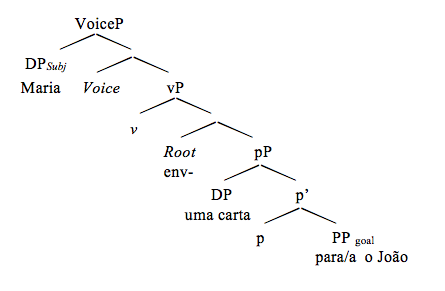
\includegraphics[width=\textwidth]{figures/calindro-img001.png}
\begin{styleBodyTextii}
\ea%15
    \label{ex:key:15}
    \gll\\
        \\
    \glt
    \z

         
\end{styleBodyTextii}

\begin{styleFootnote}
The transitive preposition as relational element can be responsible for holding a thematic relation between the DO and the IO. As such, this crucially confirms \citegen{Cuervo2010} proposal according to which ditransitive verbs do not require two separate arguments, but select a \textit{relation} between DO and the IO. For \citet{Cuervo2010}, this relation can be introduced in the argument structure by an applicative head, a small clause or a prepositional phrase.
\end{styleFootnote}

\begin{styleFootnote}
As argued before, BP does not have applicative heads in its argument structure, as it cannot express morphologically dative case anymore, as EP does. Additionally, I am assuming IOs in the relevant structures are introduced by transitive prepositions. Consequently, the oblique complement is introduced via a \textit{p}P in the argument structure. Therefore, the EP applicative construction \REF{ex:key:6} was reanalyzed in BP as \REF{ex:key:15}.
\end{styleFootnote}

\textbf{3.1.} \textbf{The} \textbf{i*} \textbf{-} \textbf{single} \textbf{argument} \textbf{introducer} \textbf{proposal}

In this section, I adopt \citet{WoodMarantz2017}’s proposal of a single argument to account for the representation of ditransitive structures with transfer, movement and creation verbs in BP. Importantly, this proposal allows us to explain the two different semantic readings conveyed by the preposition \textit{para} in sentences with creation verbs, as we will see in section 3.2. However, to understand the characteristics of this single argument introducer, I will first analyze ditransitive sentences with transfer and movement verbs which have just been discussed in the previous section.

\citet{WoodMarantz2017} propose the main heads which add participants to the event (\textit{Voice,} \textit{low} \textit{applicative,} \textit{little} \textit{p,} \textit{prepositions} \textit{(P),} \textit{high} \textit{applicative}) can be reduced to one i* single argument introducer. In these terms, three of the basic heads are defined in \REF{ex:key:16}, depending on the syntactic contexts they occur:

\ea%16
    \label{ex:key:16}
    \gll\\
        \\
    \glt
    \z

          a. Little p (figures): Bare \textit{i*} that merges with a PP.

  b. Voice (agents): Bare \textit{i*} that merges with a vP.

  c. Low appl (possessors): Bare i* that merges with a DP.

                                                                  (\citealt{WoodMarantz2017}:258)

  The introducer i* is a categorically unspecified head that does not start the derivation with a categorical feature, its categorial feature is valued by the categorial feature of the first constituent it merges with as result of a combination of an unvalued category (CAT) which may or may not trigger Merge with a constituent of category D, such as: \{[CAT: \_\_]. [S: D]\}. The underscore indicates an unvalued CAT feature and i* would be the notation for this feature bundle. The selectional features are annotated in brackets, P\textsubscript{[S: D],} for instance,\textsubscript{}  is a head of category P that selects (S) for a constituent of category D (\citealt{WoodMarantz2017}:257). Hence, the main purpose of i* is to close off the extended projection of the first constituent with which it merges (cf. 17). 

For instance, when PP merges with i*, its categorical feature of i* is valued as p, and the semantic interpretation of the preposition depends on the root. The preposition \textit{in} is different from \textit{on}, because the root ${\surd}$IN has the semantics of \textit{container} while ${\surd}$ON of \textit{surface.} Hence, the authors’ proposal for a sentence as ‘\textit{the} \textit{car} \textit{on} \textit{the} \textit{road’} is as follows:

  

 
%%please move the includegraphics inside the {figure} environment
%%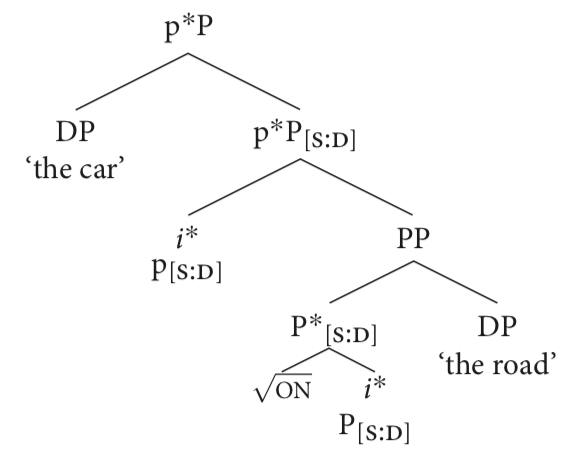
\includegraphics[width=\textwidth]{figures/calindro-img002.png}

\ea%17
    \label{ex:key:17}
    \gll\\
        \\
    \glt
    \z

         

 (Wood \& Marantz, 2017: 259)

The difference between this analysis and the one represented in \REF{ex:key:15} is the way the preposition is treated in relation to the argument it introduces. In the previous account, the preposition was only related to the Ground, not the Figure (cf.15). Under this new view, the preposition is a root that merges with i* to establish different semantic conditions for its complement, so under this view it is possible to represent the different semantics prepositions may convey. The lower i*, when merged with ${\surd}$ON, for example, assigns the DP \textit{the} \textit{road} the ${\theta}${}-role associated with it, so that the DP is interpreted as a \textit{surface}. Finally, in \REF{ex:key:17}, the highest i* is merged with the pP and then with the DP, assigning to it the idea of Figure, associated to the element in SpecpP. 

In BP, in the structures of verbs of transfer and movement, the default semantics of the prepositions \textit{a} and \textit{para} is of Goal/Recipient\footnote{\textrm{\textit{Para}} \textrm{can also be Beneficiary}\textrm{ }\textrm{whereas} \textrm{\textit{a}} \textrm{cannot, for more details cf. \citet{Calindro2015}.}}. I assume the representation of these constructions can also be realized via i*. Hence, the derivation of sentence \REF{ex:key:1}, represented in \REF{ex:key:18}, is the following: the categorial preposition \textit{para} merges with i* and then adjoins to the DP  \textit{o} \textit{João} projecting a PP. Assuming that the DO-theme \textit{uma} \textit{carta} is analogous to the DP-Figure \textit{the} \textit{road} presented in \REF{ex:key:17} merged in Specp*P, p introduces a DO in its specifier. Additionally PP is capable of denoting a transfer of possession between DO and IO - \textit{o} \textit{João}. Next, if the denotes an event which implies an agent, v introduces such a DP – \textit{Maria.} Hence, v*P consists of an i* attached to vP and then p is attached to i* merged with pP, forming p*P.

 
%%please move the includegraphics inside the {figure} environment
%%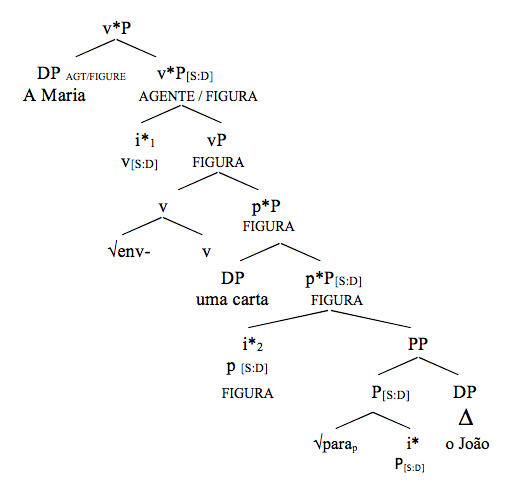
\includegraphics[width=\textwidth]{figures/calindro-img003.png}

\ea%18
    \label{ex:key:18}
    \gll\\
        \\
    \glt
    \z

        

\begin{styleHTMLPreformatted}
In the next section, we will see that the representation with i* is capable of maintaining the two beneficiary interpretations that can be instantiated by \textit{para} with creation verbs in BP.
\end{styleHTMLPreformatted}

\textbf{3.2.} \textbf{An} \textbf{analysis} \textbf{for} \textbf{ditransitive} \textbf{sentences} \textbf{with} \textbf{creation} \textbf{verbs} 

In an attempt to propose a representation that can account for creation verbs as well as movement and transfer verbs, Marantz (2009, 2013) proposes that the DOs of creation verbs can be interpreted as eventualities, as they represent the object resulting from an action. In sentence \REF{ex:key:19}, the author suggests the cake is an event itself, as it was once a group of ingredients and then becomes a final product after the action of someone making it.

The IO can be interpreted as benefitting from this change of state event that the DO has gone through \citep[156]{Marantz2013}. Hence, in \REF{ex:key:19}, there is a possession relation between the DO – \textit{John} – and the IO – \textit{a} \textit{cake}, as there would be between the DO and the IO in a DOC in English or in the sentence represented in \REF{ex:key:11} from BP. Besides, the DO is also the beneficiary of \textit{Mary’s} \textit{baking}:

 
%%please move the includegraphics inside the {figure} environment
%%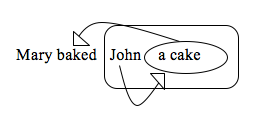
\includegraphics[width=\textwidth]{figures/calindro-img004.png}

\ea%19
    \label{ex:key:19}
    \gll\\
        \\
    \glt
    \z

         

Therefore, sentence \REF{ex:key:2} in BP can project a similar structure to \REF{ex:key:15}, given in \REF{ex:key:20}. Because, following Marantz’s view, creation verbs can also be interpreted as dynamic events are. Hence, creation verbs can be represented in the same way movement and transfer verbs are (cf. 20):

\ea%20
    \label{ex:key:20}
    \gll\\
        \\
    \glt
    \z

        

 
%%please move the includegraphics inside the {figure} environment
%%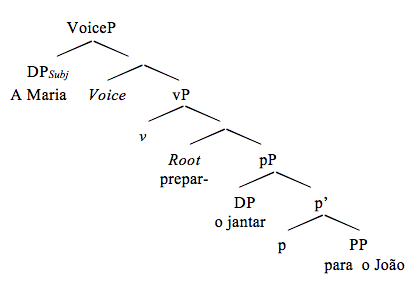
\includegraphics[width=\textwidth]{figures/calindro-img005.png}

This representation, however, does not account for the two semantic readings conveyed to the DP \textit{o} \textit{João}: \textit{beneficiary} \textit{of} \textit{the} \textit{theme} \textit{–} ‘dinner’, which would be the low applicative reading; or \textit{beneficiary} \textit{of} \textit{the} \textit{event} of \textit{Maria} having prepared dinner, which would be the high applicative.

\citet{WoodMarantz2017} distinguish \textit{little} \textit{p,} \textit{Voice,} and \textit{low} \textit{applicatives} from \textit{PP} and \textit{high} \textit{applicatives} because the latter convey semantics of their own, independently from the element they attach to. Therefore, \textit{PP} and \textit{high} \textit{applicatives} are i* heads with which lexical roots are merged. Hence, the high applicatives function as a root-adjoined i*, since the ${\theta}${}-role it assigns to the DP in its specifier is not implied by the vP semantics. Therefore, the ${\theta}${}-roles related to the high applicative are the same introduced by prepositions - Beneficiary and Locative. 

This is particularly interesting for creation verbs whose IOs have semantics of \textit{beneficiary}. In essence, a high applicative projection is like a vP because it also closes off the projection of the root, and not of the applicative head it creates. In addition, all elements that can select a vP can also select a high applicative. Therefore, when the IO is the Beneficiary of the event its semantics is of a high applicative. 

As argued previously, BP does not have applicatives, so the IOs are introduced through a prepositional phrase. Since i* is able to adjoin to a p, also following the idea that creation verbs are dynamic events as well, as discussed before. Additionally, it must be established that, according to Acedo-\citet{Matéllan2010}, prepositions function as any other lexical categories that have a neutral root and a category that determines the functional head. Hence, prepositions can be prepositional roots with categorial features that will adjoin to an i* and generate a pP (cf. 21). 

\begin{styleHTMLPreformatted}
In \REF{ex:key:21}, the categorial preposition \textit{para} merges with i* and then adjoins to the DP  \textit{João} projecting a pP. Next, i* merges with vP, valuing its categorial feature as v, projecting v* \textsubscript{[S, D]}. Finally, the DP \textit{Maria} is merged, closing off the v*P. Consequently, the interpretation of \textit{João} as the Beneficiary of the theme is conveyed, i.e., he is the one who dinner was prepared for.
\end{styleHTMLPreformatted}

\ea%21
    \label{ex:key:21}
    \gll\\
        \\
    \glt
    \z

        

 
%%please move the includegraphics inside the {figure} environment
%%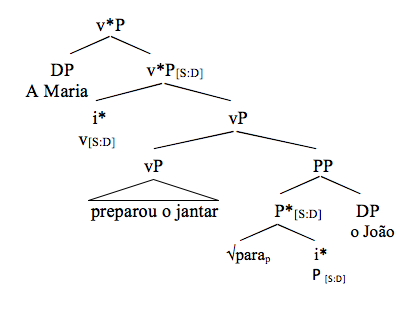
\includegraphics[width=\textwidth]{figures/calindro-img006.png}
\begin{styleHTMLPreformatted}
In the second interpretation (cf. 22) \textit{–} dinner may be appreciated by people other than \textit{João}, which is why \textit{João} is the \textit{beneficiary} \textit{of} \textit{the} \textit{event}, i.e., \textit{João} is the beneficiary of the event of \textit{Maria} preparing dinner, and will not necessarily eat it. For example, \textit{João} should prepare dinner, but he is sick, so \textit{Maria} will do it for him\footnote{ \textrm{I would like to thank an anonymous reviewer who suggested these semantic readings should be made clearer for those not familiar with BP.} }.
\end{styleHTMLPreformatted}

\bfseries

 
%%please move the includegraphics inside the {figure} environment
%%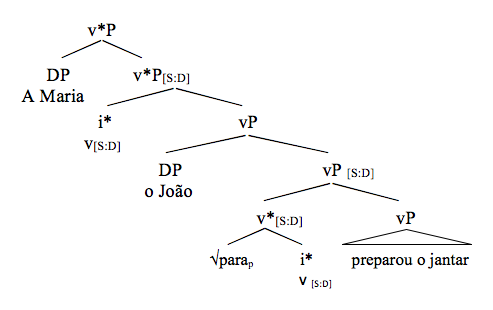
\includegraphics[width=\textwidth]{figures/calindro-img007.png}

\ea%22
    \label{ex:key:22}
    \gll\\
        \\
    \glt
    \z

        

\begin{styleHTMLPreformatted}
The prepositional root in \REF{ex:key:20} is a neutral category. Thus, if i* merges the prepositional root with a neutral feature, it generates v*, not p*, which, when merged with vP, values the categorical feature of v by projecting vP\textsubscript{[S: D].} Subsequently, the categorial feature of D is checked by merging vP \textsubscript{[S: D]} with the DP \textit{João}. Similarly, the external argument \textit{Maria} is added to the structure. Therefore, this representation captures the interpretation of a \textit{high} \textit{applicative}, since the argument \textit{o} \textit{João} is related to the event, which is the second possible interpretation for sentence \REF{ex:key:2}.
\end{styleHTMLPreformatted}

\textbf{4.} \textbf{Final} \textbf{Remarks} 

In this paper, I analyzed a change in progress in the introduction of IOs in ditransitive sentences in BP. With dynamic verbs of transfer and movement, the preposition \textit{a} is substituted by transitive preposition \textit{para} in spoken varieties of BP, however in written register they co-occur in modern BP. Hence the preposition \textit{a} and \textit{para} have the same status of a transitive prepositions, which are relational elements. This change coupled with the loss of the 3\textsuperscript{rd} person dative clitics \textit{lhe(s)} accounts for a change in the representation of ditransitive sentences, when BP is compared to other Romance languages and, in particular, to EP.

On this basis, I proposed that the argument structure of ditransitive sentences in BP does not entail applicative heads, as other Romance languages do. Hence, in this language, the relation between the DO and the IO selected by the verbal root is introduced in the argument structure by a pP. 

This representation, however, does not capture the two semantic readings that the IO introduced by \textit{para} with creation verbs can have. As such, the representation of creation verbs should necessarily involve the single argument introducer i*, with which it is possible to provide a more accurate account for both interpretations conveyed by the preposition~\textit{para~}in these contexts.\footnote{ \textrm{I would like to express my gratitude to Alice Corr, who proofread this paper.} }
\begin{verbatim}%%move bib entries to  localbibliography.bib
@book{Acedo-Matellán2010,
	address = {Barcelona},
	author = {Acedo-Matellán, Víctor},
	note = {(Doctoral Dissertation.)},
	publisher = {Universitat de Barcelona},
	sortname = {Acedo-Matellan, Victor},
	title = {\textit{Argument} \textit{Structure} \textit{and} \textit{the} \textit{Syntax-Morphology} \textit{Interface:} \textit{A}   \textit{Case} \textit{Study} \textit{in} \textit{{Latin}} \textit{and} \textit{Other} \textit{Languages}},
	year = {2010}
}


Alsina, Alex \& Mchombo, Sam. 1993. Objects asymmetries and the Chichewa Applicative   Construction. In Mchombo, Sam (ed.), \textit{Theoretical} \textit{aspects} \textit{of} \textit{Bantu} \textit{grammar}. CSLI   Publications. 50-93.

@book{Baker1988,
	address = {\textit{Incorporation:} \textit{a} \textit{Theory} \textit{of} \textit{Grammatical} \textit{Function} \textit{Changing.} Chicago},
	author = {Baker, Mark},
	publisher = {Chicago University Press},
	year = {1988}
}


@misc{Berlinck1997,
	author = {Berlinck, Rosane},
	note = {In II   Encontro do CelSul.  Anais, UFSC, Florianópolis.},
	title = {Sobre a realização do objeto indireto no português do Brasil},
	year = {1997}
}


@article{BiberauerBiberauer2015,
	author = {Biberauer, Theresa and Roberts, Ian},
	journal = {\textit{Cambridge} \textit{Occasional} \textit{Papers} \textit{in} \textit{Linguistics}},
	pages = {1--31},
	title = {Rethinking formal hierarchies: {{A}} proposed   unification},
	volume = {7},
	year = {2015}
}


@book{Calindro2015,
	address = {[Introducing arguments: the case of   ditransitives in Brazilian Portuguese]. São Paulo},
	author = {Calindro, Ana},
	note = {(Doctoral   Dissertation).},
	publisher = {University of São Paulo},
	title = {\textit{Introduzindo} \textit{Argumentos:} \textit{uma} \textit{proposta} \textit{para} \textit{as} \textit{sentenças}   \textit{ditransitivas}   \textit{do} \textit{português} \textit{brasileiro}},
	year = {2015}
}


@book{Calindro2016,
	address = {Introducing indirect arguments},
	author = {Calindro, Ana},
	note = {In   \textit{Rivista} \textit{di} \textit{Grammatica} \textit{Generativa} \textit{38}. 35-44.},
	publisher = {the locus of a diachronic change},
	year = {2016}
}


@book{CarvalhoCarvalho2018,
	address = {In \textit{Pronomes:} \textit{morfossintaxe} \textit{e} \textit{semântica}. Salvador},
	author = {Carvalho, Janayna and Calindro. Ana},
	note = {UFBA. 91-110.},
	publisher = {Ed},
	title = {A unified account for the loss of third person   clitics in {Brazilian Portuguese}},
	year = {2018}
}


@book{Chomsky1981,
	address = {Dordrecht},
	author = {Chomsky, Noam},
	publisher = {Foris Publications},
	title = {\textit{Lectures} \textit{on} \textit{government} \textit{and} \textit{binding}},
	year = {1981}
}


@book{Chomsky1986,
	address = {New York},
	author = {Chomsky, Noam},
	publisher = {Praeger},
	title = {\textit{Knowledge} \textit{of} \textit{Language}},
	year = {1986}
}


@article{Chomsky2005,
	author = {Chomsky, Noam},
	journal = {\textit{Linguistic} \textit{Inquiry}},
	pages = {1--22},
	title = {Three Factors in Language Design},
	volume = {36},
	year = {2005}
}


@misc{Cuervo2003,
	author = {Cuervo, Cristina},
	note = {MIT. (Doctoral Dissertation).},
	title = {\textit{Datives} \textit{at} \textit{large}},
	year = {2003}
}


@article{Cuervo2010,
	author = {Cuervo, Cristina},
	journal = {\textit{Probus,}},
	pages = {151--180},
	title = {Against Ditransitivity},
	volume = {22},
	year = {2010}
}


@article{DiaconescuDiaconescu2007,
	author = {Diaconescu, Constanta and Rivero, Maria Luisa},
	journal = {\textit{Probus}},
	pages = {171–195},
	title = {An applicative analysis of double object   constructions in Romanian},
	volume = {19},
	year = {2007}
}


\begin{styleDefault}
Figueiredo Silva, Maria Cristina. 2007. A perda do marcador dativo e algumas das suas consequências. [The loss of the dative marker and some consequences]. In Castilho, Ataliba \& Torres Morais, Maria Aparecida \& Lopes, Ruth \& Cyrino, Sonia (eds.), \textit{Descrição,} \textit{história} \textit{e} \textit{aquisição} \textit{do} \textit{português} \textit{brasileiro.} Fapesp, Campinas: Pontes Editores, 85-110.
\end{styleDefault}

@book{Freire2005,
	address = {[Third person anaphoric accusative and dative in Brazilian and European writing]. Rio de Janeiro},
	author = {Freire, Gilson},
	note = {(Doctoral Dissertation).},
	publisher = {UFRJ},
	title = {\textit{A} \textit{realização} \textit{do} \textit{acusativo} \textit{e} \textit{do} \textit{dativo} \textit{anafórico} \textit{de} \textit{3ª.} \textit{pessoa} \textit{na} \textit{escrita} \textit{brasileira} \textit{e} \textit{lusitana}},
	year = {2005}
}


@book{Galves2018,
	address = {[Still on Brazilian Portuguese Pronouns]. In: Medeiros, Alessandro Boechat \& Nevins, Andrew (orgs.), \textit{O} \textit{apelo} \textit{das} \textit{árvores:} \textit{estudos} \textit{em} \textit{homenagem} \textit{à} \textit{Miriam} \textit{Lemle.} Campinas},
	author = {Galves, Charlotte},
	publisher = {Pontes},
	title = {Ainda sobre os pronomes do português brasileiro},
	year = {2018}
}


Kato, Mary. 2005. Gramática do letrado: questões para a teoria gramatical. In Marques, Maria   \& Koller, Erwin (eds.), \textit{Ciências} \textit{da} \textit{Linguagem:} \textit{trinta} \textit{anos} \textit{de} \textit{investigação} \textit{e} \textit{ensino}.   Braga.   CEHUM. 131-145

Kato, Mary \& Cyrino, Sonia \& Corrêa, Vilma. 2009. Brazilian Portuguese and the recovery   of lost clitics through schooling. In Pires, Acrisio \& Rothman, Jason. (eds.),   \textit{Minimalist} \textit{Inquiries} \textit{into} \textit{Child} \textit{and} \textit{Adult} \textit{Language} \textit{Acquisition}. Mouton de Gruyter.   245–272.

@article{Larson1988,
	author = {Larson, Richard},
	journal = {\textit{Linguistic} \textit{Inquiry}},
	pages = {335--391},
	title = {On the double object construction},
	volume = {19},
	year = {1988}
}


Marantz, Alec. 1993. Implications of asymmetries in double object constructions. In   Mchombo, Sam (ed.), \textit{Theoretical} \textit{aspects} \textit{of} \textit{Bantu} \textit{grammar}. 113-151.

Marantz, Alec. 2009 Resultatives and re-resultatives: Direct objects may construct events by   themselves. Paper presented at Penn Linguistics Colloquium.

\begin{stylePreformatted}
@book{Marantz2013,
	address = {Verbal argument structure},
	author = {Marantz, Alec},
	note = {In \textit{Lingua} \textit{130.} 152-},
	publisher = {Events and participants},
	year = {2013}
}

\end{stylePreformatted}

\begin{stylePreformatted}
168.
\end{stylePreformatted}

@misc{Pylkkänen2002,
	author = {Pylkkänen, Liina},
	note = {MIT. (Doctoral Dissertation).},
	title = {\textit{Introducing} \textit{Arguments}},
	year = {2002}
}


\begin{styleNormalWeb}
@misc{Pujalte2010,
	author = {Pujalte, M.},
	note = {ms. Universidad Nacional del Comahue},
	title = {Construcciones com y cin aplicativos em el español del Rio da la Plata y el português brasileño},
	year = {2010}
}

\end{styleNormalWeb}

@misc{Scher1996,
	author = {Scher, Ana Paula},
	note = {[Constructions with two complements in English and Brazilian Portuguese]},
	title = {\textit{{As}} \textit{Construções} \textit{com} \textit{Dois} \textit{Complementos} \textit{no} \textit{Inglês} \textit{e} \textit{no} \textit{{Português}} \textit{do} \textit{Brasil}},
	year = {1996}
}


Campinas: Unicamp. (MA Dissertation).

@book{Silveira1999,
	address = {Florianópolis},
	author = {Silveira, Gessilene},
	note = {(Doctoral Dissertation).},
	publisher = {UFSC},
	title = {\textit{A} \textit{realização} \textit{variável} \textit{do} \textit{objeto} \textit{indireto} \textit{(dativo)} \textit{na} \textit{fala} \textit{de} \textit{Florianópolis}},
	year = {1999}
}


\begin{styleCorpo}
@book{Svenonius2003,
	address = {Limits on P},
	author = {Svenonius, Peter},
	note = {falling in holes, \textit{Nordlyd,} \textit{31}. 431-445.},
	publisher = {filling in holes vs},
	year = {2003}
}

\end{styleCorpo}

\begin{styleCorpo}
Svenonius, Peter. 2004. Adpositions, particles and the arguments they introduce In  Reuland, Eric \& Bhattacharya, Tammoy \& Spathas, Giorgos (eds.), \textit{Argument}   \textit{Structure.} Philadelphia: John Benjamins.  63–103.
\end{styleCorpo}

Talmy, Leonard. 1978. Figure and ground in complex sentences. In Greenberg, Joseph (ed.),   \textit{Universals} \textit{in} \textit{human}   \textit{language}.Stanford University Press. 625-649.

Torres Morais, Maria \& Berlinck, Rosane. 2006 “A caracterização do objeto indireto no português: aspectos sincrônicos e diacrônicos” [The characterization of the indirect object in Portuguese: synchronic and diachronic aspects]. In Lobo, Tania \& Ribeiro, Ilza \& Carneiro, Zenaide \& Almeida, Norma (eds.), \textit{Novos} \textit{dados,} \textit{novas} \textit{análises}. EDUFBA. 73-106.

\begin{styleFootnote}
Torres Morais, Maria \& Berlinck, Rosane. 2007.  ‘Eu disse pra ele’ ou ‘Disse-lhe a ele’: A expressão do dativo nas variedades brasileira e europeia do português”. [‘Eu disse para ele’or ‘Disse-lhe a ele’: the dative expression in Brazilian and European Portuguese varieties]. In Castilho, Ataliba \& Torres Morais, Maria \& Lopes, Ruth \& Cyrino, Sônia (eds.), \textit{Descrição,} \textit{história} \textit{e} \textit{aquisição} \textit{do} \textit{português} \textit{brasileiro}. Campinas: Ed. Pontes.
\end{styleFootnote}

@book{TorresMorais2007,
	address = {[Datives]. São Paulo},
	author = {Torres Morais, Maria},
	note = {(Professorship Thesis).},
	publisher = {USP},
	title = {\textit{Dativos}},
	year = {2007}
}


@article{TorresMoraisTorres Morais2010,
	author = {Torres Morais, Maria and Salles, Heloísa},
	journal = {\textit{Probus}},
	pages = {181--209},
	sortname = {Torres Morais, Maria and Salles, Heloisa},
	title = {Parametric change in the grammatical   encoding of indirect objects in {Brazilian Portuguese}},
	volume = {22},
	year = {2010}
}


@book{Wood2012,
	address = {New York},
	author = {Wood, Jim},
	note = {(Doctoral Dissertation).},
	publisher = {New York   University},
	title = {{Icelandic} {Morphosyntax} and Argument Structure},
	year = {2012}
}


@misc{WoodWood2017,
	author = {Wood, Jim and Marantz, Alec},
	note = {In D’Alessandro, Roberta \& Franco, Irene \& Gallego, Ángel (orgs.), \textit{The} \textit{Verbal} \textit{Domain}. Oxford University Press. 255-278.},
	title = {The Interpretation of External Arguments},
	year = {2017}
}


\end{verbatim}
\sloppy\printbibliography[heading=subbibliography,notkeyword=this]
\end{document}
